\documentclass[11pt]{article}
\usepackage[margin=1.5cm]{geometry}
\usepackage{amsmath,amssymb}
\usepackage{enumitem}
\usepackage{tikz}
\usepackage{listings}
\usepackage[T1]{fontenc}
\setlength{\columnsep}{0.7cm}
\setlength{\parindent}{0pt}
\setlist{nosep,leftmargin=*}
\lstset{
  basicstyle=\ttfamily\scriptsize,
  columns=fullflexible,
  keepspaces=true,
  aboveskip=2pt,
  belowskip=2pt,
  frame=single,
  breaklines=true
}

\begin{document}
\twocolumn

\title{Chapter 13 Warm-Up: The Diamond Inheritance Problem}
\author{Prof. Jordan C. Hanson}
\date{\today}
\maketitle

\section{A Diamond-Shaped Class Hierarchy}

Suppose we begin with a general \texttt{Student} class:

\begin{verbatim}
class Student:
    def describe(self):
        return "Student"
\end{verbatim}

Now create two child classes:

\begin{verbatim}
class Course(Student):
    def describe(self):
        return "Course group"
class Major(Student):
    def describe(self):
        return "Major group"
\end{verbatim}

Both \texttt{Course} and \texttt{Major} inherit from \texttt{Student}, but each \textbf{overrides} the same method.

Finally, define

\begin{verbatim}
class College(Course, Major):
    pass
\end{verbatim}

The inheritance pattern forms a diamond:

\begin{center}
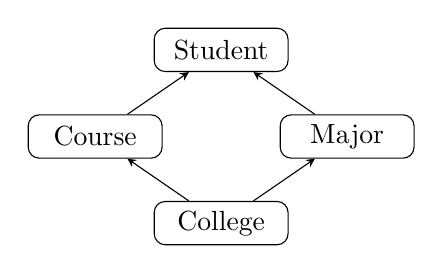
\begin{tikzpicture}[
  box/.style={draw, rounded corners, minimum width=1.7cm,
              minimum height=0.55cm, align=center},
  >=stealth
]
\node[box] (student) at (0,2.2) {Student};
\node[box] (course) at (-1.6,1.1) {Course};
\node[box] (major) at (1.6,1.1) {Major};
\node[box] (college) at (0,0) {College};

\draw[->] (course) -- (student);
\draw[->] (major) -- (student);
\draw[->] (college) -- (course);
\draw[->] (college) -- (major);
\end{tikzpicture}
\end{center}

\textbf{Question:} Why might the method
\texttt{describe()} appear ambiguous for a
\texttt{College} object?

\vspace{0.25cm}

\section{Which Method Runs?}

Create an object:

\begin{verbatim}
wc = College()
print(wc.describe())
\end{verbatim}

Before running the code, predict the output.  There are two possible inherited versions:

\begin{verbatim}
Course.describe()
Major.describe()
\end{verbatim}

Python must decide which one has priority.

\section{Method Resolution Order}

Python resolves multiple inheritance using the
\textbf{Method Resolution Order}, or \textbf{MRO}.

Try:

\begin{verbatim}
print(College.mro())
\end{verbatim}

For

\begin{verbatim}
class College(Course, Major):
\end{verbatim}

Python searches classes according to the MRO.

Which class is checked first after \texttt{College}?  Which class is checked next? Therefore, which version of \texttt{describe()} should run?

\section{Reverse the Parent Order}

Now change the class definition to

\begin{verbatim}
class College(Major, Course):
    pass
\end{verbatim}

Predict:

\begin{verbatim}
wc = College()
print(wc.describe())
\end{verbatim}

What changed?

\vspace{0.3cm}

\textbf{Key idea:} In multiple inheritance, Python uses the MRO to
decide which inherited method to call when more than one parent
provides a method with the same name.

\end{document}
